In den folgenden Kapiteln wird die ausgewählte Hardware des Projekts vorgestellt. Dabei wird zuerst auf die technischen Merkmale eingegangen und dann auf den genauen Verwendungszweck im Projekt. 

\subsection{Raspberry PI}        
\label{sec:Raspberry PI-1} 


\subsubsection{Vorstellung des Raspberry PI}        
\label{sec:Vorstellung des Raspberry PI-1} 

Das Raspberry PI ist ein Einplatinencomputer, den es in verschiedenen Ausführungen gibt. Je nach Ausführung variieren die Ausstattungsmerkmale. Zu den Grundsätzlichen Ausstattungsmerkmalen gehören eine CPU, unterschiedlich viel RAM und eine iGPU Einheit. Er wurde von der Raspberry PI Foundation entwickelt und hatte das ursprüngliche Ziel einen günstigen Computer für den Schulunterricht bereitzustellen. Daher ist es auch möglich eine vollständige Linux Distribution als Betriebssystem zu nutzen und es wurde sogar eine speziell angepasste Distribution veröffentlicht, die Raspbian bezeichnet wird. 
Aufgrund der verschiedenen Möglichkeiten wird er aber mittlerweile auch in vielen anderen Anwendungsgebieten genutzt. Insbesondere die neueren Modelle, die mit mehreren USB Ports, \ac{GPIO} Pins, einem Ethernet Port und weiteren Anschlüssen ausgestattet sind, werden auch in verschiedensten Projekten privater Personen genutzt. Ein weiteres Merkmal ist die Größe des Raspberry PI's, die mit maximal 93mmx63.5mmx20mm sehr klein ausfällt. Zusätzlich gibt es diverses, bereits für den Raspberry PI ausgelegtes, Zubehör, welches weitere Erweiterungsmöglichkeiten bietet. So gibt es Kameras, Gehäuse, kleine Displays und WLAN Sticks, die den Funktionsumfang erweitern. So wurden bereits diverse Projekte vorgestellt, die zeigen, dass die Einsatzmöglichkeiten des Raspberry Pis wesentlich größer sind. (vgl. \cite{.28.12.2016} \cite{.28.01.2017})
\\
\begin{figure}[!htb]
	\centering
	\includegraphics[scale=0.5]{Raspberry-Pi-2-web.png}
	\caption[RaspberryPi Modell 2 B]{RaspberryPi Modell 2 B+,\\ Quelle: https://www.raspberrypi.org/wp-content/uploads/2016/02/Raspberry-Pi-2-web.jpg}
\end{figure}


\subsubsection{Verwendung im Projekt}        
\label{sec:Verwendung des Raspberry PI-1} 
Der Raspberry PI wird für das Projekt genutzt, um einen zentralen Server bereitzustellen. Aufgrund der technischen Merkmale kann zeitgleich ein Webserver und ein Datenbankserver betrieben werden. Zudem kann über die USB Anschlüsse ein WLAN Stick angeschlossen werden, sodass die Buttons über das WLAN Netzwerk des Raspberry PIs zum zentralen Server kommunizieren können. Dazu muss mithilfe eines Skriptes der WLAN Stick von einem Empfänger zu einem Sender bzw. Access Point umfunktioniert werden. Um die dann eingehenden Nachrichten der Buttons empfangen zu können, muss zudem noch ein entsprechendes Skript im Hintergrund laufen, dass die Daten empfängt. Aufgrund von mehreren parallel laufenden Prozessen (Webserver, Datenbankserver, WLAN Skript und Skripte zum Empfangen der Daten) wird einiges an Rechenleistung benötigt, die der Raspberry Pi allerdings aufbringen kann. 

Der Webserver auf dem Raspberry Pi wird dabei sowohl für das Frontend als auch für das Backend benötigt werden. Das Frontend soll dem Nutzer die Möglichkeit geben, die Liste von Waren zu verwalten und die Buttons zu konfigurieren bzw. Hilfestellung zur Einrichtung zu geben. Das Backend des Servers wird unter anderem aus einer \ac{REST} \ac{API} bestehen, die sowohl die Anfragen des Webservers verarbeitet als auch die Anfragen an die Datenbank im allgemeinen. 
Der Datenbankserver im Hintergrund wird die benötigte Datenbank entsprechend verwalten. 
\newpage

\subsection{``Pretzelboard''}        
\label{sec:Pretzelboard-1} 
\subsubsection{Vorstellung des ``Pretzelboard''}        
\label{sec:Vorstellung des ``Pretzelboard''} 
Das ``Pretzelboard'' ist ein sogenanntes Elektronikmodul, dass unter verschiedenen Namen bekannt ist. Neben ``Pretzelboard'' ist der Name ``NanoESP-Board'' ebenfalls bekannt. Die Besonderheit des Boards ist ein bereits angeschlossenes WLAN Modul, welches sowohl als Sender als auch Empfänger arbeiten kann. 

Da es zudem den gleichen Microcontroller wie das bekanntere Microcontrollerboard ``Arduino Uno'' nutzt, kann die Entwicklungsumgebung von Arduino zur Entwicklung von Software genutzt werden. 
Der Vorteil der bereits erfolgten Kombination und Verdrahtung von WLAN Modul und Microcontroller des Pretzelboards liegt darin, dass der Nutzer dies nicht mehr machen muss und somit wesentlich weniger Kenntnisse vorausgesetzt werden müssen. (vgl. \cite{.b}\cite{.kafka}\cite{FranzisVerlagGmbH.27.11.2015})

\begin{figure}[!htb]
	\centering
	\includegraphics[scale=0.4]{Pretzel.jpg}
	\caption[``Pretzelboard'']{``Pretzelboard'',\\ Quelle: http://cdn.pollin.de/article/xtrabig/X880281.2.JPG}
\end{figure}

\subsubsection{Verwendung im Projekt}        
\label{sec:Verwendung des ``Pretzelboard''} 
Das ``Pretzelboard'' wird im Projekt als Button genutzt. Sowohl die kleine Größe als auch die bereits vorhandene WLAN Funktionalität sorgen dafür, dass sich das Board dafür besonders gut eignet. Aufgrund der Tatsache, dass es sich bezüglich der Programmierung nicht von einem Arduino Board unterscheidet, besteht die Möglichkeit, dass auf das Wissen und den Support einer bereits größeren Community zurückgegriffen werden kann. 

Da sich das Board zudem auf ein Elektroniksteckboard setzen lassen kann, ist auch die Verbindung mit einem Button und Statusleuchten möglich. Nach der erfolgreichen Montage kann dann das entsprechende Programm aufgespielt werden und bei vorhandener Stromversorgung kann die entsprechende Nachricht über das WLAN Netzwerk an den Empfänger gesendet werden. Das Pretzelboard kommuniziert diese Nachricht mithilfe des zuvor bereits erwähnten Protokolls \ac{UDP} (vgl. Kapitel \ref{sec:UDP-1}).


\begin{figure}[!htb]
	\centering
	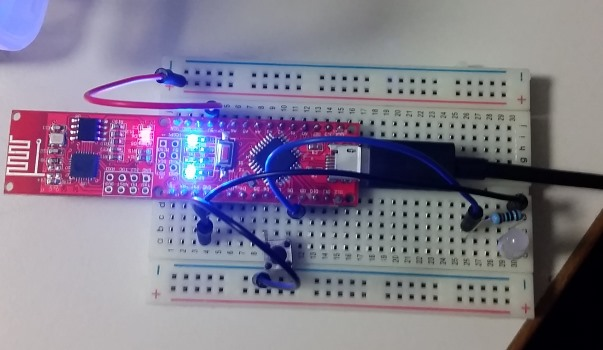
\includegraphics[scale=0.6]{Pretzel_Projekt.jpg}
	\caption[Pretzelboard im Projekt]{Pretzelboard im Projekt,\\ Quelle: Eigene Aufnahme}
\end{figure}

%Bild vom fertigen Button
\newpage

\subsection{ESP8266 Lua}
\label{sec:ESP8266}

\subsubsection{Vorstellung des ESP8266 Lua}        
\label{sec:Vorstellung des ESP8266} 

Der ESP8266 Lua ist ein Entwicklungsboard, welches bereits ein integriertes WLAN Modul besitzt und mit einem \ac{TCP}/\ac{IP} Stack ausgestattet ist. Einer der vorgesehenen Einsatzzwecke ist unter anderem das Internet of Things. Das Board kann zudem mit Steckbrett arbeiten und bietet daher ähnliche Möglichkeiten, wie das bereits erwähnte \nameref{sec:Pretzelboard-1}. Zudem ist es möglich, dass die Software für das ESP8266 Lua Entwicklungsboard ebenfalls über die Arduino \ac{IDE} entwickelt werden kann. Allerdings sind technische Unterschiede zum Pretzelboard vorhanden, was dazu führt, dass andere Treiber genutzt werden müssen. 
Diese können nachinstalliert werden und stehen dann zur Nutzung des Boards bereit. (vgl. \cite{Carius.15.01.2017}\cite{.d})

\begin{figure}[!htb]
	\centering
	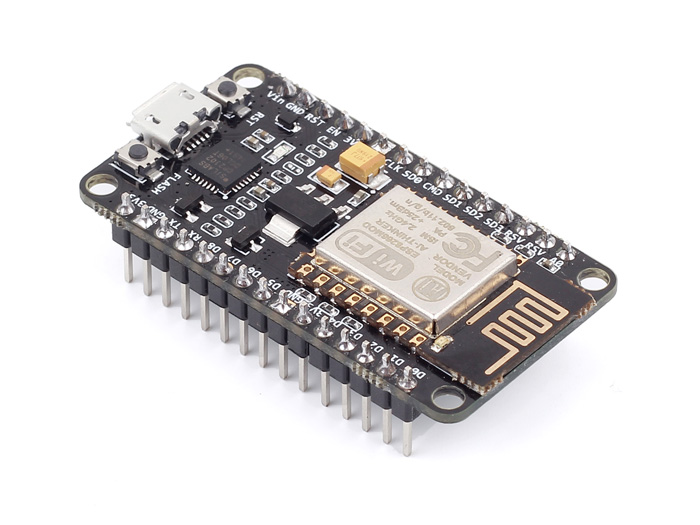
\includegraphics[scale=0.4]{ESP.jpg}
	\caption[ESP8266]{ESP8266,\\ Quelle: https://www.roboter-bausatz.de/media/image/dc/14/6e/113990105-1.jpg}
\end{figure}

\subsubsection{Verwendung im Projekt}        
\label{sec:Verwendung des ESP8266} 
Das Board wird im Rahmen des Projektes als weiterer Button genutzt. Es bietet sich für diese Funktion an, da es ebenfalls recht klein ist und alle benötigten Funktionen bereits vorhanden sind. Neben den vorhandenen Funktionen ist auch die Möglichkeit vorhanden, dass eine bereits durch das Pretzelboard bekannte Entwicklungsumgebung genutzt werden kann. Das bietet die Möglichkeit, dass statt des \ac{UDP} Protokolls das bereits erwähnte \nameref{sec:TCP-1} Protokoll ausprobiert werden kann. 
Der Aufbau des Boards soll ebenfalls durch ein Elektroniksteckboard umgesetzt werden. Dazu wird das Board auf eben dieses Steckboard gesetzt und mit einem Button, Statusleuchten und entsprechenden Kabeln verbunden. Nach der Betätigung des Buttons wird das Board geweckt und eine Funktion schickt ein entsprechendes Datenpaket an einen Empfänger.
\begin{figure}[!htb]
	\centering
	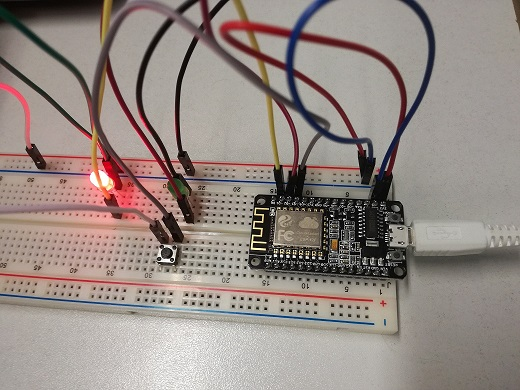
\includegraphics[scale=0.5]{ESP_Projekt.jpg}
	\caption[ESP8266 im Projekt]{ESP8266 im Projekt,\\ Quelle: Eigene Aufnahme}
\end{figure}
\newpage


 

%Bild vom fertigen Button 

\subsection{Amazon Dash Button}
\label{sec:Amazon Dash Button}

\subsubsection{Vorstellung des Amazon Dash Buttons}        
\label{sec:Vorstellung des Amazon Dash Buttons} 
Am 31.08.16 wurde der Amazon Dash Button offiziell in Deutschland exklusiv für Prime Mitglieder eingeführt (vgl. \cite{ONLINE.31.08.2016}).
Dabei handelt es sich um einem mit dem WLAN verbundenen Button, mit welchem sich zum Großteil Verbrauchsartikel per Knopfdruck bestellen lassen.
Jeder Button wird mit einem Produkt verknüpft, das während des Einrichtens ausgewählt wird.
Sollte nun das Produkt zur Neige gehen oder gar aufgebraucht sein, so kann der Nutzer den Button drücken und es wird sofort ein Bestellvorgang eingeleitet.
Weitere Interaktion seitens des Nutzers ist dabei nicht notwendig.

Der Dash Button wird über die Amazon App auf einem Android- oder iOS-Smartphone eingerichtet und verwaltet und funktioniert an allen Orten mit einer WLAN-Verbindung.
Sobald die Einrichtung abgeschlossen ist, wird eine Benachrichtigung (sofern aktiviert) an das Smartphone versendet, immer wenn eine Bestellung aufgegeben wurde (vgl. \cite{.dash}).
Zusätzlich verfügt der Button über einen Bestellschutz.
Mit dieser Funktion gibt der Dash Button keine Bestellung auf, bis die vorherige Bestellung geliefert wurde – egal wie oft der Dash Button gedrückt wird.
Der Amazon Dash Button ist in Deutschland für aktuell 4,99  \euro  erhältlich (Stand: 17.05.17).
Jedoch wird dieser Preis mit der ersten Bestellung verrechnet, wodurch dem Kunden keine zusätzlichen Kosten entstehen.

\begin{figure}[!htb]
	\centering
	
\includegraphics[scale=0.5]{Dash.jpg}
	\caption[Amazon Dash Button für Produkte von Ariel]{Amazon Dash Button für Produkte von Ariel,\\ Quelle: https://images-eu.ssl-images-amazon.com/images/I/41SMHhklQYL.\_A
	C\_US218\_.jpg}
\end{figure}

\subsubsection{Untersuchung des Amazon Dash Buttons}
\label{sec:Untersuchung des Amazon Dash Buttons}
Die Untersuchung des Amazon Dash Buttons bezieht sich nur auf dessen Funktionen.
Die Hardware wurde nicht analysiert, da diese bereits mehrfach, auch auf unterschiedlichen Websites analysiert wurde (vgl. \cite{.17.05.2017}\cite{.17.05.2017b}).

Der Amazon Dash Button wird einem kleinen braunen Karton geliefert.
Dieser enthält neben dem Button noch 2 Dokumente, eine Gebrauchsanleitung und Sicherheitsinformationen.
Die Gebrauchsanleitung beschreibt nur den Download der Amazon App sowie die schritte, die notwendig sind um den Konfigurationsassistenten zu starten.

Die eigentlich Einrichtung läuft dann wie folgt ab:
Zuerst müssen WLAN und Bluetooth auf dem Gerät aktiviert werden.
Danach muss der Amazon Dash Button für ca. 6 Sekunden gedrückt werden, bis dieser Blau leuchtet.
Dann muss der Benutzer auf seinem Smartphone auf "`Verbinden"' drücken.
Die Amazon App versucht sich dann via Bluetooth mit dem Button zu verbinden.
Sollte dies erfolgreich sein, so kann der User das  Produkt auswählen, welche auf dem Button hinterlegt werden soll.

Hierbei hat der Benutzer hier nur auf eine sehr kleine Auswahl des Herstellers Zugriff.
So gibt es beispielsweise bei dem "`Power Point Energy Drink Dash Button"' nur eine Auswahl aus 4 Produkten:
\begin{itemize}
\item Power Point Energy Drink Classic, 24er Pack (24 x 250 ml)
\item Power Point Energy Drink Himbeere, 24er Pack (24 x 250 ml)
\item Power Point Energy Drink Waldmeister, 24er Pack (24 x 250 ml)
\item Power Point Energy Drink Ice Blue , 24er Pack (24 x 250 ml) 
\end{itemize}
Hat der Benutzer seine Auswahl getroffen, muss er noch den Dash Button mit einem WLAN Netzwerk verbinden.
Dabei sucht der Dash Button nach verfügbaren Netzwerken welche dann dem Benutzer in der Amazon App angezeigt werden.
Nun muss der Benutzer nur noch ein WLAN Netzwerk auswählen, das Passwort für dieses eingeben und schon kann der Button benutzt werden.

\subsubsection{Verwendung des Amazon Dash Buttons im Projekt}
\label{sec:Verwendung des Amazon Dash Buttons im Projekt}
Der Amazon Dash Button konnte erfolgreich in das Projekt eingebunden werden. Hierbei waren jedoch ein paar Workarounds notwendig, welche in \ref{sec:Einbindung des Amazon Dash Buttons-1} näher ausgeführt werden. Dabei funktioniert der Dash Button genauso wie die selbst einwickelten Button.
%Bild vom Button 
\newpage